% ============================================================================
\section{Evaluation and responsible deployment}
% ============================================================================

\begin{frame}{Evaluating TTS quality}
  \begin{itemize}
    \item \textbf{Human tests:} Does the voice sound natural?
    \item \textbf{Similarity:} Is the generated speech close to real speech?
    \item \textbf{Intelligibility:} Can speech-to-text systems understand it?
    \item \textbf{Cloning:} How well does it copy a specific voice?
    \item TTS is evaluated by playing a sentence to human listeners and having them
give a mean opinion score (MOS) on a scale of 1 to 5.
  \end{itemize}
\end{frame}

\begin{frame}{Objective Evaluation}
  \begin{itemize}\itemsep0.4em
    \item Human MOS panels are slow and expensive, so large-scale development leans on objective proxies.
    \item \textbf{Intelligibility:} transcribe the synthesized speech with a strong ASR model and compute WER against the input text.
    \item \textbf{Speaker similarity:} cosine similarity between speaker embeddings of the reference prompt and the generated audio.
    \item \textbf{Predicted MOS:} neural predictors (UTMOS, NISQA) estimate human scores from audio alone.
    \item Modern systems score close to human recordings, so plain MOS saturates; side-by-side comparative MOS (CMOS) separates systems better.
  \end{itemize}
\end{frame}

\begin{frame}{Voice Cloning Safeguards}
  \begin{itemize}\itemsep0.4em
    \item \textbf{Consent and disclosure:} clone only with the speaker's permission and label synthetic audio as synthetic.
    \item \textbf{Watermarking:} embed an inaudible signature in generated audio so it can be identified later (AudioSeal).
    \item \textbf{Detection:} train classifiers to spot synthetic speech; the Voicebox authors report a highly effective classifier for their own outputs.
    \item These mitigations are partial: watermarks do not survive every re-encoding, detectors lag the newest generators, and neither the Voicebox model nor its detector was publicly released.
  \end{itemize}
\end{frame}

\begin{frame}{Ethics before you collect speech}
  \centering
  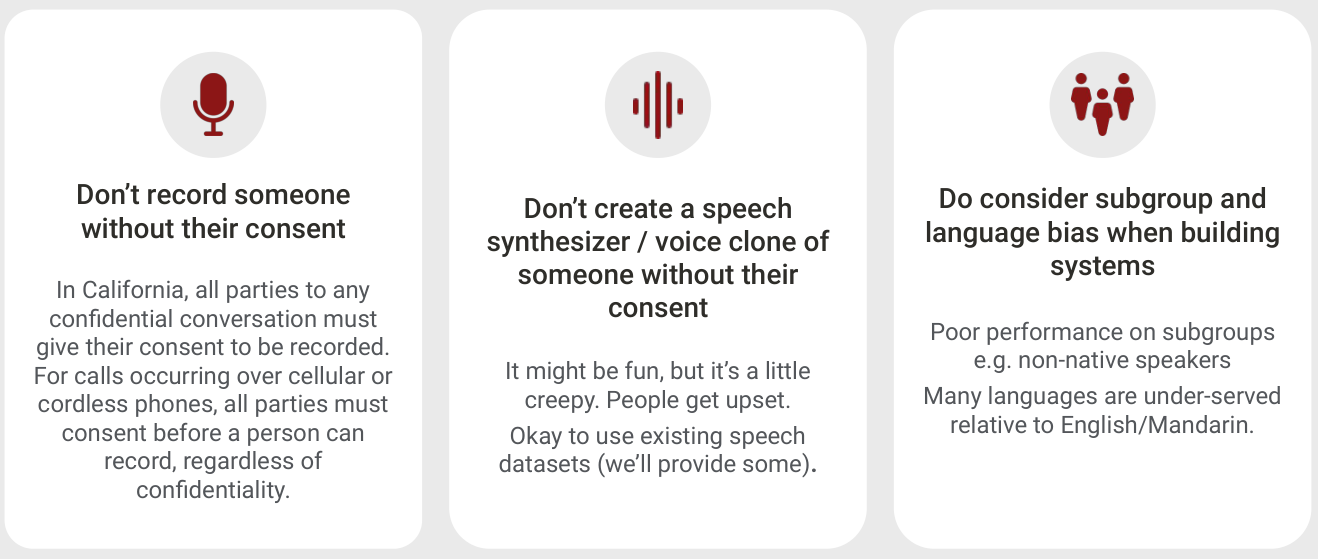
\includegraphics[width=\textwidth,height=0.62\textheight,keepaspectratio]{images/tts/tts_ethics_guidelines.png}
  \slideimgsource{Stanford CS224S, Lecture 1 (2024 Spring), slide 8.}
\end{frame}

\begin{frame}{Takeaways}
  \begin{itemize}
    \item One text can be spoken many ways (speed, stress, intonation). Most systems still go {text $\rightarrow$ acoustic features $\rightarrow$ waveform}; newer models like VALL-E predict {audio tokens} directly.
    \item TTS improved in stages: {stitch recorded clips} $\rightarrow$ {slow but high-quality} neural models (Tacotron~2, WaveNet) $\rightarrow$ {faster parallel} models (FastSpeech~2, HiFi-GAN, VITS) $\rightarrow$ {foundation models} that clone voices from a short sample (VALL-E, Voicebox).
    \item {Voice cloning} from a few seconds of audio works well today, but can fail on rare accents; use it carefully with {consent, labeling, and fake-speech detection}.
  \end{itemize}
\end{frame}
